\documentclass[]{article}
\usepackage[]{algorithm2e}
\usepackage{amsmath}
\usepackage{framed}
\usepackage{tabularx}
\usepackage[dutch]{babel}
\usepackage{graphicx}
\usepackage{epstopdf}
\usepackage{mcode}
\usepackage{enumitem}


%opening
\title{Practicum NMB : Eigenwaardenproblemen}
\author{Matthijs van Keirsblick en Harald Sch\"{a}fer}
\date{vrijdag 25 april 2015}

\newcommand{\opgave}[1]{\pagebreak\section*{Opgave #1}}


\begin{document}

\maketitle
\opgave{1}


We beginnen door een QR-factorisatie te berekenen van $A_{0}$ met eender welke methode. Vervolgens berekenen we $b = Q^{*}*b_{0}$. Met deze waarden kunnen we de iteratieve berekening starten die hieronder beschreven staat. De $G_{x}$ matrices zijn givens transformaties om de toegevoegde rijen van K terug op nul te stellen om zo terug een bovendriehoeksmatrix R te bekomen waarin de nieuwe waarden in verwerkt zijn.


\begin{framed}
\begin{algorithm}[H] 
 $Q^{(0)}*R^{(0)} = A_{0}$\\
 $b = Q^{(0)*}*b_{0}$\\
 \For{i = 1 to k}{
  $f = n*d$\\
  $R^{(i)} = G_{f}^{*}*...*G_{1}^{*}*
  \begin{bmatrix}
    	R^{(i-1)}	\\
    	K
    \end{bmatrix}$\\
  $R^{(i)} = R^{(i)}(:n,:)$\\
  $Q^{(i)} = I*G_{1}*...*G_{f} $\\
  $b^{(i)} = Q^{(i)*}*
  \begin{bmatrix}
      	b^{(i-1)}	\\
      	c
      \end{bmatrix}$\\
  $b^{(i)} = b^{(i)}(:n,:)$\\
 }
 
% \caption{How to compute incremental least squares solution with QR factorisation}
\end{algorithm}
\end{framed}

\noindent Aan het einde van elke iteratie is het mogelijk om $x^{(i)}$ te berekenen door achterwaardse substitutie toe te passen op de vergelijking $R^{(i)}*x^{(i)} = b^{(i)}$. Omdat na elke iteratie maar $R^{(i)}$ en  $b^{(i)}$ opgeslagen moet worden is het duidelijk dat het gebruikte geheugen niet toeneemt. Omdat de grootte van de matrices R en b niet toeneemt neemt het rekenwerk ook niet toe met elke iteratie. Voor het berekenen van een Givens-transformatie zijn 2 delingen, 2 vermenigvuldigen, een optelling en een vierkwantswortel nodig. Er moeten n*d Givens-transformaties berekend worden per iteratie. Een vermenigvuldiging met een rotatiematrix van grootte n+d zoals in dit geval vraagt 4*n vermenigvuldigingen en 2*n optellingen. Er gebeuren n*d van die matrix vermenigvuldigingen voor de berekening van $R^{(i)}$ en n*d-1 voor de berekening van $Q^{(i)}$. Tot slot  gebeurt er nog voor de berekening van de $b^{(i)}$ een matrix vermenigvuldiging waarvoor $(n+d)^2$ vermenigvuldigingen gebeuren en $(n+d-1)*(n+d)$ optellingen.

\begin{itemize}
  \item $n*d*2$ delingen
  \item $n*d$ vierkantswortels
  \item $n*d*2 + 2*n*(2*n*d-1) + (n+d-1)*(n+d) \approx 4*n^2*d$ optellingen
  \item $n*d*4 + 4*n*(2*n*d-1) + (n+d)^2 \approx 8*n^2*d$ vermenigvuldigingen
\end{itemize}


\opgave2
\begin{enumerate}[label=\alph*)]

\item Een norm van een vector is minimaal wanneer die vector de nulvector is.
Dat betekent dat $||Ax-\rho x||_{2}$ minimaal is wanneer $x \rho = Ax$ (scalaire vermenigvuldiging is commutatief). We kunnen deze vergelijking oplossen naar $\rho$ door het te zien als een kleinste kwadraten probleem waarbij Ax een gekende vector is, x een gekende matrix/vector en $\rho$ is de onbekende. We vermenigvuldigen de vergelijking links met $x^T$ en bekomen $x^{T}x \rho = x^{T}Ax$. Omdat $x^{T}x$ een scalar is kunnen we hierdoor delen wat ons brengt naar $\rho = \frac{ x^{T}Ax}{x^{T}x}$. Dit is inderdaad het Rayleigh quoti\"{e}nt.\\

\noindent
\item Als $\mu$ naar $\lambda(i)$ gaat, wordt het stelsel meer singulier, dus het conditiegetal van $A-\mu I$ groter. Dit betekent dat perturbatiefouten zwaar doorwegen. Deze perturbatiefouten worden echter alleen versterkt in de richting van de vector die we zoeken en in alle andere richtingen verzwakt. Hierdoor blijft de iteratie nog steeds doorgaan in de richting van de juiste eigenvector en blijft de fout beperkt.
\end{enumerate}

%\section{}

\opgave{3}
Alvorens de QR methode, al dan niet met shifts, toe te passen op de matrix, moeten we hem omzetten naar Hessenberg vorm. Deze omzetting kost ons \'{e}\'{e}nmaal \textit{O}($n^3$) rekenwerk. \\
Omdat de Hessenberg vorm al bijna bovendriehoeks is, kan de QR factorisatie in minder stappen uitgevoerd worden, namelijk in \textit{O}($n^2$) in plaats van in \textit{O}($n^3$). Deze factorisatie moet in iedere iteratie van de QR methode uitgevoerd worden, dus  de vermindering in rekenwerk is erg significant. Figuur ~\ref{opgave3} toont de structuur van de  Hessenbergvorm van mat1.

\begin{figure}[h]
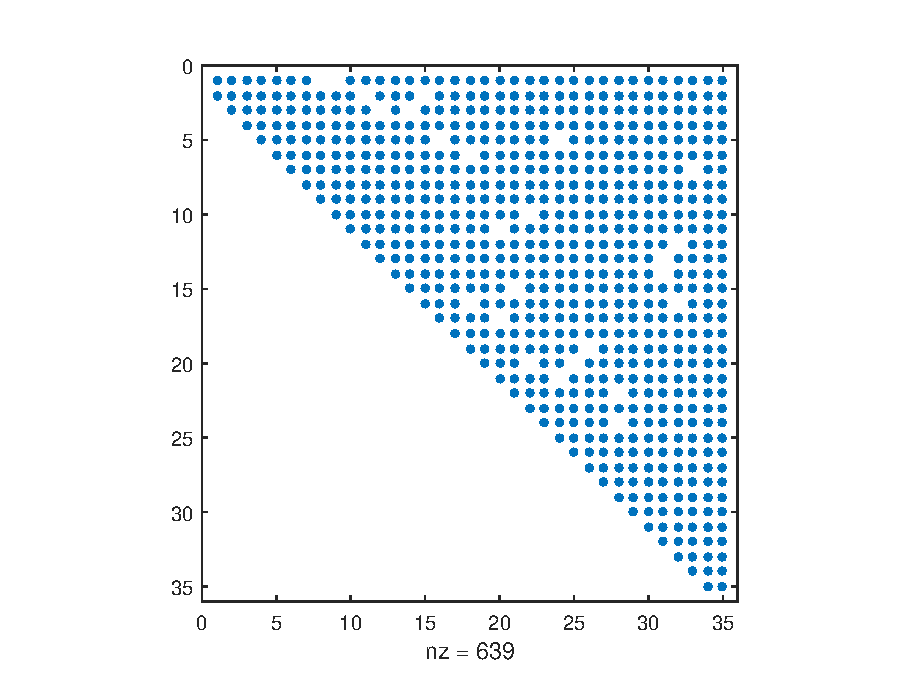
\includegraphics[width=1\textwidth]{opgave3.eps}
\caption{De structuur van de Hessenbergvorm van mat1}
\label{opgave3}
\end{figure}

\opgave{4}

De verwachting vanuit de theorie is dat de QR methode zonder shifts traag convergeert, zoals power- iteratie. De QR methode met shifts zou in het slechtste geval niet(Rayleigh shifts) of kwadratisch (Wilkinson shifts) convergeren. In figuur ~\ref{opgave41} en tabel ~\ref{opgave42} worden het benodigde aantal iteratiestappen voor de berekening van \'{e}\'{e}n eigenwaarde per methode weergegeven, samen met de fout op het tussenliggende resultaat. We merken op dat  zowel de Rayleigh Shift als de Wilkinson Shift zorgen voor een kubische convergentie (aantal beduidende cijfers $* 3$ in iedere stap). 
De Wilkinson Shift heeft in dit geval een snellere convergentie door een (toevallig) goedgekozen eerste shiftwaarde. De convergentiefactor voor de eerste stap van de Wilkinson shift methode is hier $3.46$, voor de Rayleigh shift methode is hij $2.827$ en voor de QR methode zonder shift is hij zelfs kleiner dan 1. Het valt op dat de QR methode zonder shift niet lijkt te convergeren op deze grafiek. Dit is wel zo, maar pas na een groot aantal stappen (niet weergegeven). Na ~40 iteratiestappen is de machinenauwkeurigheid bereikt. 

\begin{figure}[h]
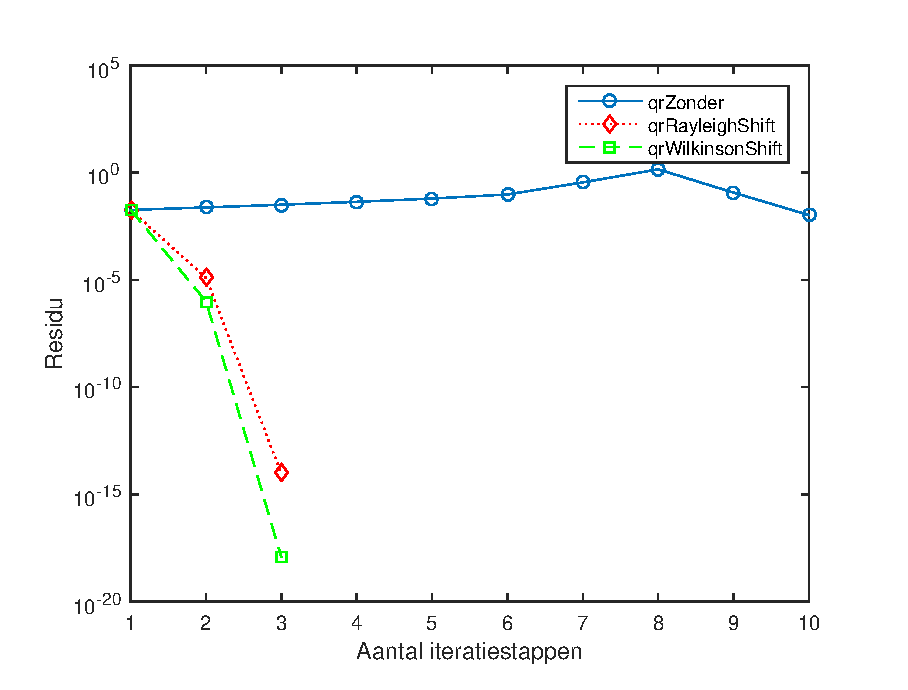
\includegraphics[width=1\textwidth]{opgave4.eps}
\caption{De fout op het berekenen van \'e\'en eigenwaarde.}
\label{opgave41}
\end{figure}

\pagebreak

\begin{table}[h]
\noindent\makebox[\textwidth]{%
\begin{tabularx}{1.3\textwidth}{l|llllllllll}
Methode&1&2&3&5&10&20&25\\\hline
QRzonder&$0.01836$ & $0.02411$ & $0.03212$ & $0.06223$ & $0.0106$ & $1.498\times 10^{-6}$ & $2.059\times 10^{-8}$ \\
QRrayleigh & $0.01836$ & $1.234\times 10^{-5}$ & $\epsilon_{mach}$ & $\epsilon_{mach}$ & $\epsilon_{mach}$ & $\epsilon_{mach}$ & $\epsilon_{mach}$ \\
QRwilkinson & $0.01836$ & $9.833\times 10^{-7}$ & $\epsilon_{mach}$ & $\epsilon_{mach}$ & $\epsilon_{mach}$ & $\epsilon_{mach}$ & $\epsilon_{mach}$\\
\end{tabularx}}
\caption{Convergentie van QR methodes voor het berekenen van \'e\'en eigenwaarde.}
\label{opgave42}
\end{table}

\paragraph{•}
Een aantal zaken zijn nog op te merken:
\begin{itemize}
	\item Voor de 2 methoden die gebruik maken van shifts, wordt in iedere stap een aantal keren een geshifte inverse iteratie gedaan, om zo het element op positie $(k,k)$ te laten convergeren naar de $k^{e}$ eigenwaarde. Opmerkzaam is dat de $i^{e}$ eigenwaarde met $i = 1,\dots,k-1$ als k het aantal eigenwaarden is dat we nog moeten berekenen, ook al genaderd wordt, terwijl het algoritme nog bezig is eigenwaarden verderop in de matrix te berekenen m.b.v shift- iteraties. Hoe kleiner i, hoe minder sterk dit effect. De oorzaak hiervan is dat de QR methode, naast inverse iteratie, ook simultane iteratie toepast.
	\item De methode met Wilkinson- shifts doet er 66 stappen over om alle eigenwaarden van mat1 te vinden tot op machineprecisie. De methode met Rayleigh- shifts doet er 83 stappen over, en die zonder shifts maar liefst 686 stappen. Wilkinson shifts vereisen iets meer berekeningen in iedere stap, maar de convergentie is beter dan bij Rayleigh shifts, omdat Wilkinson shifts rekening houden met het symmetrische eigenwaarden. Rayleigh shifts kunnen in zo'n gevallen zorgen voor een trage (of zelfs onbestaande) convergentie.
\end{itemize}


\opgave{5}


Figuur~\ref{opgave5} toont de convergentie van de besproken methodes. Aangezien we hier de gelijktijdige iteratie uitvoeren met I als de start matrix is deze methode hetzelfde als de QR methode zonder shifts. Deze convergeert dus linear net zoals de methode van de machten. De QR methode met rayleigh quotient shift convergeert cubisch. Deze methode is eigenlijk dezelfde methode als de rayleigh iteratie, maar dan in Matrix vorm. Daarom is het ook logisch dat het convergentiegedrag analoog is.
Het nadeel van Rayleigh iteratie is dat je convergeert naar een eigenwaarde die in de buurt ligt van de gekozen startwaarde. Het is niet mogelijk om alle eigenwaarden en eigenvectoren van een matrix te berekenen zonder al een redelijke schatting van iedere eigenwaarde te hebben.

\begin{figure}[h]
\noindent 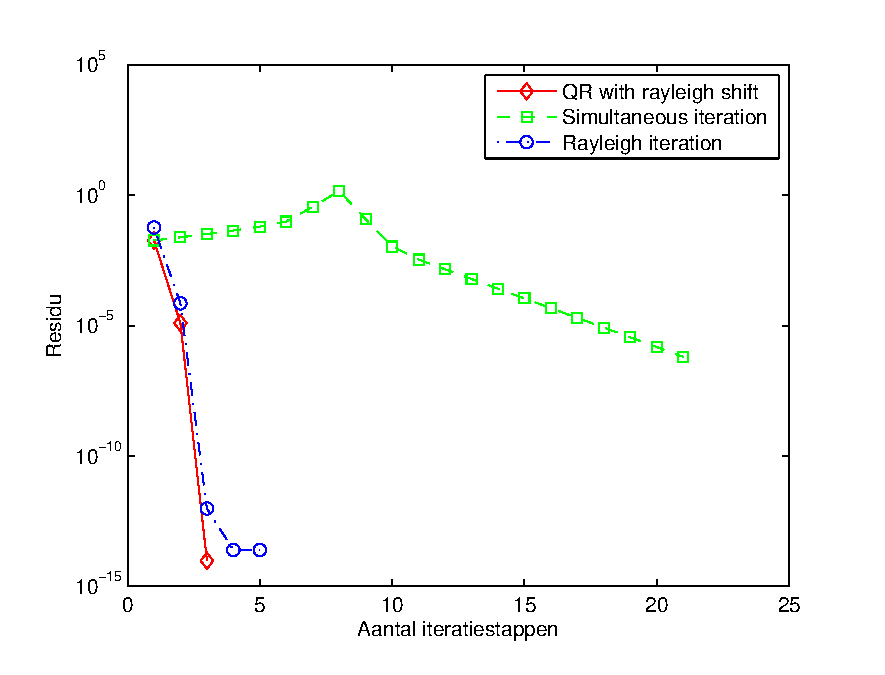
\includegraphics[width=1\linewidth]{opgave5.eps}
\caption{Convergentie van rayleigh iteratie, QR methode met rayleigh shifts en simultane iteratie naar \'{e}\'{e}n eigenwaarde}
\label{opgave5}
\end{figure}

\opgave{6}

De Arnoldi methode berekent iteratief de eigenwaarden van een matrix A. Dit gebeurt door een Hessenberg matrix te maken van A, die in iedere stap groter wordt. De eigenwaarden van die groeiende matrix, de zogenaamde ritz waarden, zijn een goede benadering voor de eigenwaarden van de matrix A. Alhoewel er in het begin veel minder ritz waarden zijn dan eigenwaarden van A, vormen de ritz waarden toch vrij snel goede benaderingen voor alle eigenwaarden. Dit is vooral effectief voor ijle matrices omdat de eigenwaarden daarvan dicht bij elkaar liggen. \'{E}\'{e}n ritz waarde is dan genoeg om meerdere eigenwaarden van A te benaderen. Alhoewel de benaderingen zeer ruw zijn met zo een klein aantal iteraties zien we toch dat we hier met maar 40 iteraties nog slechts een gemiddelde fout hebben van 10 $\%$. Dit is niet weinig, maar we hebben dit wel met weinig rekenwerk kunnen vinden. In figuur~\ref{opgave6} zien we ook dat de 20 grootste eigenwaarden beter benaderd worden door de ritz waarden. Dit is omdat de ritz waarden sneller convergeren naar de uitschieters. 
\linebreak Er valt op te merken dat willekeurige $n\times n$ matrices \'{e}\'{e}n eigenwaarde hebben die ongeveer n keer de gemiddelde waarde van de elementen van die matrix is, terwijl alle andere eigenwaarden rond 0 gegroepeerd zijn. De Arnoldi methode zal heel snel convergeren naar die uitschieter, die meestal de meest interessante eigenwaarde is. 

\begin{figure}[h]
\noindent \includegraphics[width=1\linewidth]{Opgave6.eps}
\caption{Convergentie}
\label{opgave6}
\end{figure}


\opgave{7}


De interlacing eigenschap zegt dat bij een symmetrische tridiagonale matrix $\lambda ^{(k+1)}_{j} < \lambda ^{(k)}_{j} < \lambda ^{(k+1)}_{j+1}$, waarbij $\lambda ^{(k)}_{j}$ de $j^{e}$ eigenwaards is van de $k^{e}$ principiele submatrix. $\lambda _{1}$ is dan de kleinste eigenwaarde van $A^{k}$ en $\lambda _{k}$ de grootste. We zullen deze eigenschap illustreren aan de hand van het volgende voorbeeld.

\begin{equation}
A=\begin{bmatrix}
    	8 & 4 & 0 & 0 & 0	\\
    	4 & 3 & -3 & 0 & 0 \\
    	0 & -3 & 9 & -2 & 0 \\
    	0 & 0 & -2 & 1 & -2 \\
    	0 & 0 & 0 & -2 & 6 
    \end{bmatrix}
    ,
    A^{1}=\begin{bmatrix}
        	8
        \end{bmatrix}
        ,
    A^{2}=\begin{bmatrix}
           	8 & 4 \\
           	4 & 3
         \end{bmatrix}
         , ...
\end{equation}
\begin{figure}[h]
\noindent 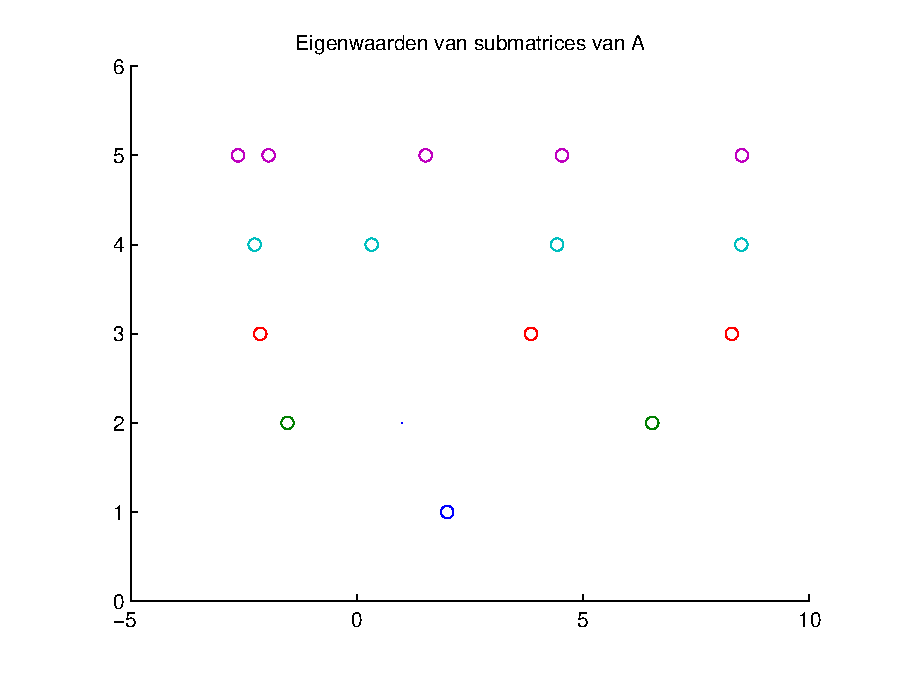
\includegraphics[width=1\linewidth]{opgave7.eps}
\caption{Interlacing}
\label{opgave71}
\end{figure}

\pagebreak 

\begin{table}[h]
\noindent\makebox[\textwidth]{%
\begin{tabularx}{0.8\textwidth}{l|llllll}
Submatrix&$\lambda _{1}$&$\lambda _{2}$&$\lambda _{3}$&$\lambda _{4}$&$\lambda _{5}$\\\hline
$A^{1}$&$2$ & $/$ & $/$ & $/$ & $/$ \\
$A^{2}$&$-1.5311$ & $6.5311$ & $/$ & $/$ & $/$\\
$A^{3}$&$-2.1330$ & $3.8478$ & $8.2852$ & $/$ & $/$\\
$A^{4}$&$-2.2544$ & $.30192$ & $4.4261$ & $8.4980$ & $/$\\
$A^{5}$&$-2.6223$ & $-1.9468$ & $1.5220$ & $4.5360$ & $8.5111$\\
\end{tabularx}}
\caption{Eigenwaarden van de principiele submatrices van A}
\label{opgave72}
\end{table}

Het is duidelijk aan de hand van de bovenstaande tabel dat de interlacing eigenschap geldt. Bijvoorbeeld $-2.1330 < -1.5311 < 3.8478 < 6.5311 < 8.2852$ voor $A^{2}$ en $A^{3}$


\opgave{8}

Algemene werkwijze om met de bisectiemethode de k-de eigenwaarde $\lambda_k$ te vinden van een symmetrische, tridiagonale matrix A van grootte m:

\begin{enumerate}
 \item Kies een interval $I=[a0,b0]$ dat $\lambda_k$ bevat.
 \item Dan geldt, gebruik makende van de Sturm sequentie en de interlace- eigenschap van eigenwaarden van opeenvolgende submatrices $A^{i}$ van A: $s(b_0) >= k$ and $s(a_0) < k$ met $s(x)$ het aantal tekenwisselingen in de Sturm sequentie met shift $x$. Hieraan moet steeds voldaan zijn. Door $b_0$ en $a_0$ te verkleinen of vergroten kunnen we het interval I laten convergeren naar de waarde van $\lambda_k$.
 \item Gebruik de bisectietechniek om het interval te verkleinen: evalueer de Sturm sequentie $p_k(a_0) = det(A^{(k)} - a*I)$ voor $k=1\dots m$ waarbij $a=(a0+b0)/2$, en tel het aantal tekenwisselingen $s$. Als \'{e}\'{e}n van de sequentiewaarden 0 is, vergelijk je de volgende waarde met de laatste waarde die niet 0 was. Voor Matlab-code, zie hieronder.
 \item Als $s >= k$, vervang $b_0$ door $(a0+b0)/2$ en herhaal de iteratie, maar nu op het kleiner interval $I=[a_0,(a0+b0)/2]$.
 Indien $s < k$, vervang $a_0$ door $(a0+b0)/2$ en herhaal.
 \end{enumerate}
 Door herhaalde iteratie en verkleinen van het inverval convergeert het algoritme naar de k-de eigenwaarde van A. Een aantal grafieken van de convergentie naar de echte eigenwaarden zijn weergegeven in ~\ref{opgave8.eps}
 
 Om nu alle eigenwaarden binnen een interval te bekomen, moeten we vinden welke eigenwaarden zich binnen dit interval bevinden.Met behulp van de Sturm sequentie en de interlacing eigenschap van de submatrices van A, kunnen we bepalen hoeveel eigenwaarden er zijn in het interval I. Het aantal eigenwaarden in het interval $ (- \infty, a_0]$ is gelijk aan het aantal tekenveranderingen in de Sturm sequentie $ p_k (a_0) = det (A ^ {(k)} - a_0 * I) $, met k=1\dots m als m de grootte is van de matrix A. De index van de eerste eigenwaarde in het interval is dan dit getal + 1. Op dezelfde manier kunnen we het aantal eigenwaarden kleiner dan $ b_0 $ bepalen. Het aantal eigenwaarden in het interval $ [a_0, b_0] $ is dan het verschil tussen de twee. We kennen dus de indices van eerste en laatste eigenwaarden in het interval I, en kunnen voor al deze indices het hierboven beschreven algoritme toepassen.

\begin{framed}
\begin{lstlisting}
function [E,residue,nbSteps] = bisection(A,a,b,tol)
% Eigenvalue of tridiagonal matrix using the bisection method
%   A       The matrix 
%   a       The lower bound of the interval
%   b       The upper bound of the interval
%   tol     The precision with which to determine the eigenvalues

%   E       The column vector with resulting eigenvalues
%   residu  The matrix with residues after each step, one row per
%   eigenvalue calculation

[p,sBeforeA0] = sturmSeq(A,a);
[p,sBeforeB0] = sturmSeq(A,b); 
 % sBeforeA0 = number of eigvals before the interval, 
 % so first eigval in interval has index sBeforeA0 + 1
nbEigInterval = sBeforeB0 - sBeforeA0;
E = zeros(nbEigInterval,1);
residue = zeros(nbEigInterval,1);
nbSteps = zeros(nbEigInterval,1);

n = size(A,1);
eigA = eig(A);

for k=sBeforeA0+1:sBeforeB0
    % bisection for locating k'th eigenvalue
    xl = a; %   lower bound
    xu = b; %   upper bound
    i = 1;  %   used for the residue
    exactLambda = eigA(k); %    this too
    x= rand(n,1);          %    this too
    
    while xu-xl >= tol
        xn = (xl+xu)*.5;
        i = i+1;
        [p,s] = sturmSeq(A,xn); % sturmSeq with shift xn, 
        						% returns nb_eigenvalues in (-inf, xn)
        residue(k - sBeforeA0,i) = norm(exactLambda*x - xn*x);
        
        if s >= k       % you counted too much, 
        				% so it's located in the first half of the interval
            xu = xn;
        else            % not enough eigvalues found yet, 
        				% search in second half of the interval
            xl = xn;
        end
    end
    
    E(k - sBeforeA0) = xn;    %save calculated eigenvalues
    nbSteps(k - sBeforeA0,1) = i;
end
\end{lstlisting}
\label{matlabBisection}
\end{framed}



\begin{framed}
\begin{lstlisting}
function [ p,s ] = sturmSeq( A, shift )
% This function returns the sequence of det(A - xI) 
% and the number of sign changes
%   A = tridiagonal matrix
%   lamb = guess eigen value (used in bisection method)
%   p = a pvector polynomials (p_1 to p_n)
%   s = the number of sign changes

n= size(A,1);
p = zeros(n,1);
s = 0; 
prevsign= 1; %p(0) = 1

% p(-1) = 0 & p(0) = 1
p(1) = (A(1,1) - shift) * 1 - 0^2 * 0;  
if sign(p(1))*prevsign < 0
    s = s+1; 
    prevsign = - prevsign;
end

p(2) = (A(2,2) - shift)*p(1) - A(1,2)^2 * 1;
if sign(p(2))*prevsign < 0
    s = s+1; 
    prevsign = - prevsign;
end

% for the rest, we can just use the formula
for k = 3:n
    % A(k,k) = a_k ; A(k,k-1) = b_k-1  because b_k-1 is the entry on 
    % the k-1'th column of row k, and a_k is the k-th entry on that row 
    % (b is offdiagonal element, a is diagonal element)
    p(k) = (A(k,k) - shift)*p(k-1) - A(k-1,k)^2 * p(k-2);     %formula (30.9)
    if sign(p(k))*prevsign < 0 
        s = s+1; 	% sign change means new eigenvalue found 
        			% in interval (-inf,shift)
        prevsign = - prevsign;
    end
end
\end{lstlisting}
\label{matlabSturm}
\end{framed}

\begin{figure}
\begin{center}
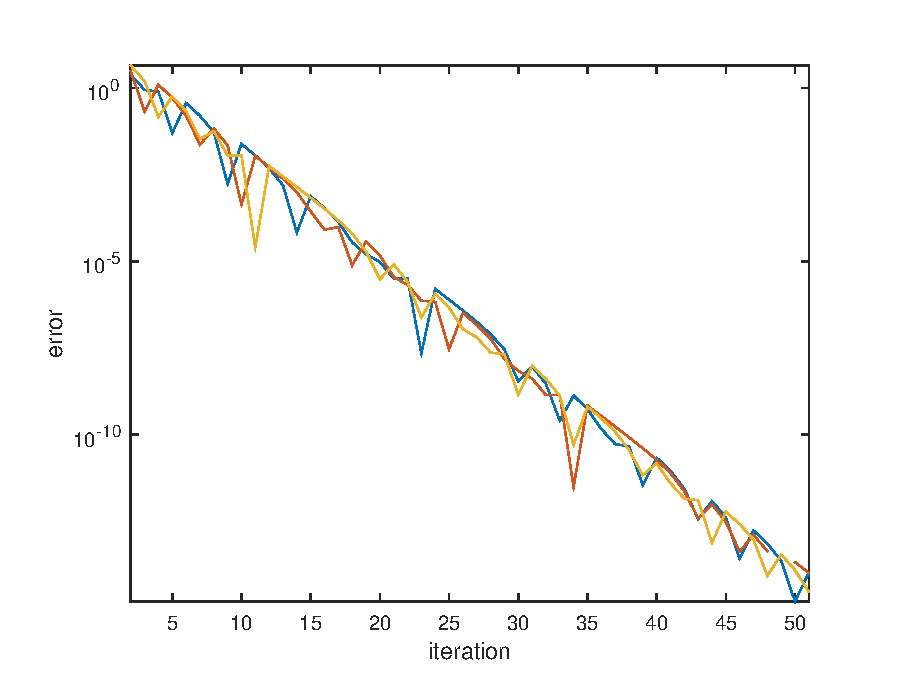
\includegraphics[width=1\textwidth]{opgave8.eps}
\end{center}
\caption{Opgave 8. Bisectiemethode: evolutie van het residu voor berekeningen van een aantal eigenwaardes}
\label{opgave8}
\end{figure}


Tests ter controle van de werking van deze Matlab- functies zijn hieronder weergegeven. In alle gevallen waarin de methode convergeert, gebeurt dit 
\begin{itemize}
	\item Een diagonale matrix met 5 gelijke eigenwaarden. Het algoritme vindt ze allemaal. Bij grote matrices van deze vorm worden vrij grote benaderingsfouten gemaakt voor de ide eigenwaarden. Bij de $i$-de eigenwaarde is de fout 2 keer zo groot als bij de $(i-1)$-de eigenwaarde. Dit komt omdat de bisectiemethode het verschil niet kan uitmaken tussen alle verschillende eigenwaarden omdat de afstanden ertussen (=0) te klein zijn.
	A\[\left[ \begin{array}{cccccc}
6 & 0 & 0 & 0 & 0 \\  
0 & 6 & 0 & 0 & 0 \\  
0 & 0 & 6 & 0 & 0 \\ 
0 & 0 & 0 & 6 & 0 \\ 
0 & 0 & 0 & 0 & 6 \\  
\end{array} \right] \]\linebreak

	\item Een diagonale matrix met allemaal verschillende positieve elementen. Bij  grotere matrices (vanaf ongeveer grootte 100) van deze vorm kunnen de opeenvolgende $p_i$'s zo in absolute waarde stijgen, dat ze na een tijd niet meer voorgesteld kunnen worden in de computer (er is geen compenserende factor $b_{k-1}^2$ in formule (30.9) in het HB, omdat de buitendiagonaalelementen allemaal nul zijn). Het algoritme vindt dan niet alle eigenwaarden.

	\item Een willekeurige matrix, die dus niet tridiagonaal is, zelfs niet symmetrisch. De bissectie methode werkt hier inderdaad niet, zoals door de theorie voorspeld.
\[	\left[	\begin{array}{ccccc}
0.88058&0.82562&0.15711&0.88857\\
0.23512&0.88369&0.62517&0.26367\\
0.24486&0.94537&0.69899&0.23479\\
0.64092&0.3908&0.085869&0.83966\\
\end{array}	\right]	\]\linebreak

	\item Een matrix die bijna tridiagonaal is, behalve \'{e}\'{e}n element. De bissectie methode werkt hier inderdaad niet, zoals door de theorie voorspelt.
	\[ \left[	\begin{array}{llllll}
3&6&0&0&0&0\\
6&3&1&0&0&0\\
0&1&3&2&0&0\\
0&0&2&3&3&0\\
0&0&0&3&3&4\\
5&0&0&0&4&3\\
\end{array}	\right] \]

	\item Gewone symmetrische tridiagonale matrices, met het zoekinterval van verschillende groottes, positief/negatief,...
\end{itemize}

\opgave{9}
We willen bepaalde eigenwaardes vinden, bijvoorbeeld de eerste 7 eigenwaardes van de matrix. Vanuit de theorie verwachten we dat de bisectiemethode een rekentijd van \textit{O}(m) nodig heeft per eigenwaarde. Eigenvectoren kunnen dan makkelijk met inverse iteratie bepaald worden in \textit{O}(m).\\
Met de QR methode moeten we meteen alle eigenwaarden (en eigenvectoren) berekenen. Dit zorgt voor een veel grotere rekencomplexiteit voor grote matrices wanneer slechts een beperkt aantal eigenwaarden en/of eigenvectoren gevraagd is.
Figuur \ref{opgave9} illustreert dat dit inderdaad het geval is.

\begin{figure}[h]
\begin{center}
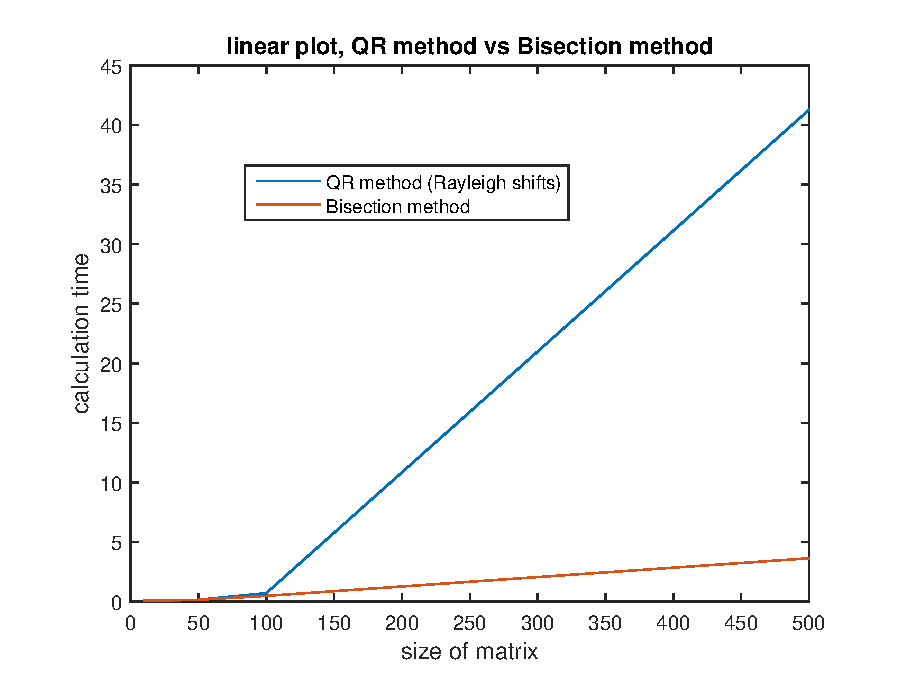
\includegraphics[width=1\textwidth]{opgave9lin.eps}
\end{center}
\caption{Opgave 9. QR en Bisectie, berekening 7 eerste eigenwaarden -en vectoren}
\label{opgave9}
\end{figure}


\end{document}
